\chapter{Development of the Automated Balance System}

\section{Development of module through OOP, managing models and controllers}

As discused before, the core elements composing a store's balance system are Balance Updates and Bank Transfers. These elements are constructed as Models, which in terms of OOP are represented by Classes. These Classes' attributes and elements will be handled independently by Models and Controllers Classes. Every action or method regarding the models will be handled by the Controllers.\\

The Controllers will generate instances of the Balance Updates and Bank Transfers models and handle the relationships between them. They will serve as the link between the application and the Database as well by using TypeORM Repositories for these Models.\\

These controllers classes handle different actions and processes within them and where designed in such way that their methods always return a specific interface as their response. This interface is called \textbf{\textit{ControllerResponse}} and it will either be a successful or unsuccessful response. This will be identified with the attribute \textit{success}. For successful responses, the attribute \textit{res} will be included and its type will be described by the generic indicator \textbf{\textit{T}}. In the other hand, for any unsuccessful response, the attribute \textit{error} will be included containg an object in the form of a \textbf{\textit{ControllerError}} as follows:

    
    \begin{verbatim}
        
        type ControllerResponse<T> =
        | {
            success: true; 
            res: T;
            }
        | {
            success: false;
            error: ControllerError;
            };
            \end{verbatim}
            
A \textbf{\textit{ControllerError}} will contain additional details as a string describing the specific exception making it compatible with Javascript's Error type:
            
    \begin{verbatim}
        interface ControllerError {
            msg: string;
            }
    \end{verbatim}
                

    \subsection{Balance Updates}

The system's general balance will be composed by numerous Balance Updates. Where the changes in the balance of the store will be reflected on each of them. As shown in Figure \ref{fig:uml_balance_update}, every instance will have its own \textit{id} as primary key, which will serve as reference for any foreign key relationship. The atribute \textit{amount} indicates exactly how the store's balance will be updated, keeping a record of the store's previous balance and the current balance after the update was added in the corresponding attributes.

\begin{figure} [H]
    \centering
    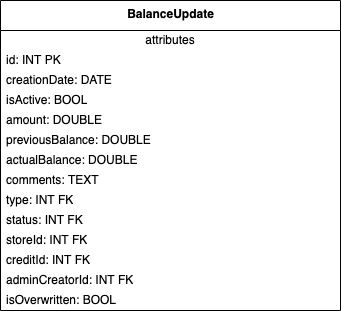
\includegraphics[scale = 0.7]{assets/uml/BalanceUpdate.png}
    \caption{Balance Update UML}\label{fig:uml_balance_update}
\end{figure}

Every Balance Update must have a \textit{storeId} foreign key, indicating which store's balance it is affecting. This is how the modularity of the balance system is defined per every individual store.\\ 

The nullable attribute \textit{creditId} will serve as a reference for linking a Credit entity to the Balance Update it created when it served as a \textit{Contribution} or \textit{Credit cancellation} to the store's balance. These refere to the types that a Balance Update could have and will be furtherly explained in the following section.\\

Some Balance Updates could be manually generated by any administrator with the appropiate permissions. For this scenario, it is important to keep a record of who made these changes by saving this administrator's id in the attribute \textit{adminCreatorId} and label these changes with the respective \textit{type}. 


\subsubsection{Balance Updates Types}

Every Balance Update will have a specific \textit{type} attribute. These types are managed as a table with static values and referenced through their \textit{id} attribute. Every Balance Update presents the same behaviour independently from their \textit{type}, nontetheless, they represent specific changes and reasons for these changes that do depend on the \textit{type} they have. For this reason, the type can not be edited once the instance of the Balance Update is generated. The different possible types of Balance Updates are described in Figure \ref{fig:balance_updates_types} 

\begin{figure}[H]
    \caption{Balance Update Types}\label{fig:balance_updates_types}
    \begin{tabularx}{1\textwidth} { 
    | >{\centering\arraybackslash}X 
    | >{\centering\arraybackslash}X 
    | >{\raggedright\arraybackslash}X | }
   \hline
   id & Type & Description \\
   \hline
   1 & \textit{Contribution} & Contribution to balance due to a new credit   \\
   \hline
   2 & \textit{Disbursement} & Disbursement generated through the confirmation of a Bank Transfer   \\
   \hline
   3 & \textit{Credit Cancellation} & Loads negative balance due to credit cancelation   \\
   \hline
   4 & \textit{Adjustment} & Loads adjustment in balance to be considered in the next Bank Transfer   \\
   \hline
   5 & \textit{Disbursement override} & Overrides the amount addedd to the balance from another Disbursement   \\
  \hline
\end{tabularx}
\end{figure}

\subsubsection{Overwriting Balance Updates}


Balance Updates have an attribute to indicate if the object was overwritten. Whenever an object is overwritten, this means that there is an additional Balance Update that is cancelling its affectation on the store’s general balance. This is particularly helpful to keep control of a store’s balance modification for those scenarios where there are involved some cancelations, overrides or any manual adjustment. The only Balance Updates that could be overwritten are those of the types of \textit{Disbursement} and \textit{Contribution}.\\

A Balance Update of type \textit{Disbursement} is generated whenever a confirmation that a Bank Transfer has been successfully accepted is received. There are some edge cases where this \textit{Disbursement} Balance Update needs to be overwritten for external reasons; this could happen, for example, due to the cancelation of a Bank Transfer. Furthermore, there is a very rare, but possible, scenario where the money could be returned even after it was confirmed, but the expected outcome is just as that of a cancellation. For these cases, the Disbursement that was generated is no longer valid, hence, an update to the store’s balance should be made. This is done by generating an additional Balance Update with type \textit{Disbursement Override} as shown in Figure \ref{fig:override_disbursement}. This new Balance Update will contribute once again the amount that was previously reduced to the store’s balance.\\

\begin{figure} [H]
    \centering
    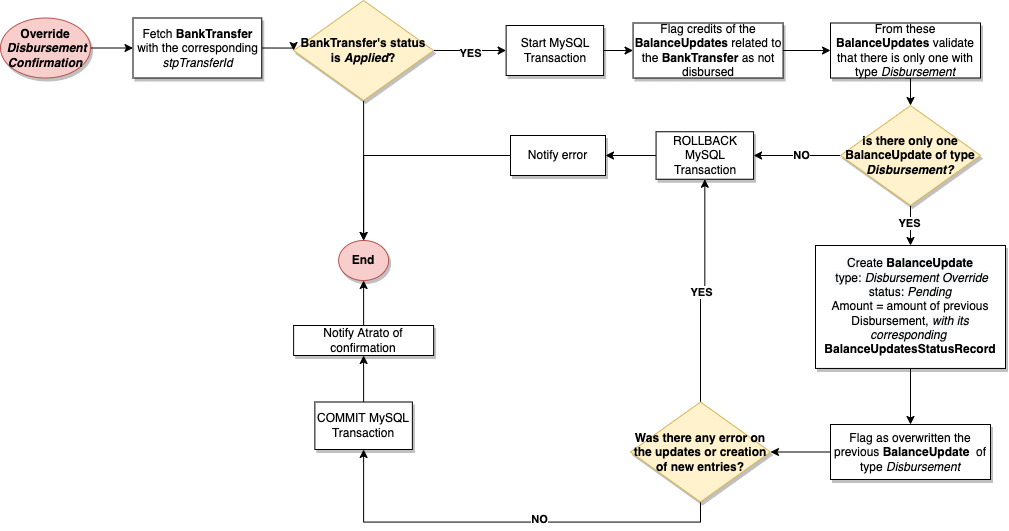
\includegraphics[scale = 0.4]{assets/diagrams/DisbursementOverride.png}
    \caption{Process for overriding a previously confirmed Balance Update of type Disbursement}\label{fig:override_disbursement}
\end{figure}


Furthermore, Balance Updates of type Contribution could also be overwritten at some point. These are created once a partner has confirmed a product’s delivery through their dashboard and the credit of that product will generate a contribution to the store’s balance. This means that there is some amount that Atrato must eventually transfer to the partner’s bank account depending on the disbursement modality that this partner has active. These contributions could eventually be overwritten if the credit is later cancelled. For this particular scenario, a new Balance Update of type \textit{Credit cancelation} needs to be created to compensate the previous contribution, regardless of the contribution’s status as shown in Figure \ref{fig:dlowchart_credit_cancelation}.


\begin{figure} [H]
    \centering
    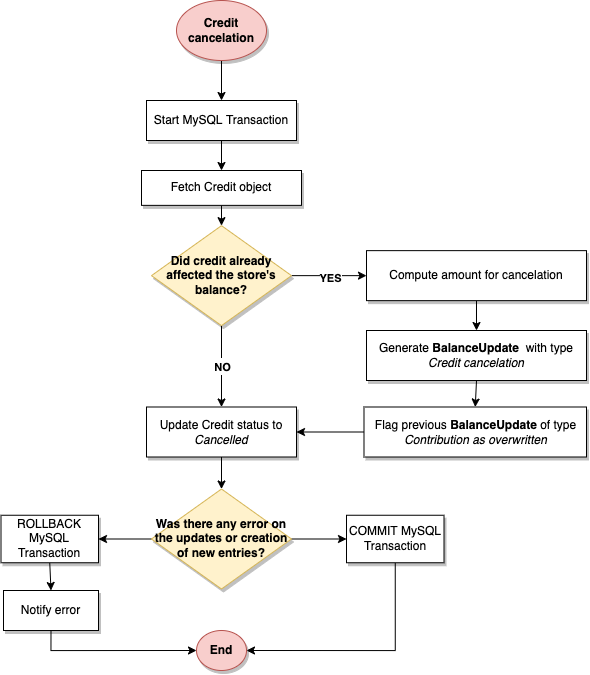
\includegraphics[scale = 0.6]{assets/flowcharts/CreditCancelation.png}
    \caption{Processing a credit's cancelation and its affectation to a store's balance system}\label{fig:dlowchart_credit_cancelation}
\end{figure}

\section{Bank Transfers}

Just as the Balance Updates, as shown in Figure \ref{fig:uml_bank_transfers}, every Bank Transfer will have their primary key \textit{id}, useful for any foreign key relationship, and a not nullable \textit{storeId}. The attribute \textit{status} will internally describe wether the Bank Transfer has already been sent, confirmed, cancelled or rejected, while the attribute \textit{stpStatus} will be the value received upon any incoming update regarding the payment order related to this Bank Transfer. The status of the Bank Transfers can not be arbitrarily updated from one status to another one, the specific expected behavoiour will be furtherly discissed in Chapter 4.
The \textit{dispersionDate} will indiacte the date when the Bank Transfer was dispatched as a payment order. This dispatch could be either done automatically or through a manual confirmation, hence, it will no necesarily be the same as the \textit{creationDate}. Furthermore, the \textit{trackingKey} will be the attribute used to link the Bank Transfers objects and the payment orders from STP.

\begin{figure} [H]
    \centering
    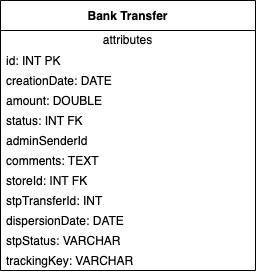
\includegraphics[scale = 0.7]{assets/uml/BankTransfers.png}
    \caption{Bank Transfer UML}\label{fig:uml_bank_transfers}
\end{figure}

\subsection{Generating Bank Transfer objects}

Once the trigger for generating a new Bank Transfer is received, the store's current balance will be used as the Bank Trasfer's amount. As shown in Figure \ref{fig:bank_Transfer_trigger}, all the Balance Updates with status \textit{Pending} will be related to the new Bank Transfer and will then update their status to \textit{In transit}. An additional confirmation could be added at this point for those stores where the Bank Transfers must be confirmed manually by the Treasury team. If this confirmation is not necessary, then a new paymenr order can be generated and sent through STP using the information of the Bank Transfer. This process will be furtherly described in Chapter 4. Once the Bank Transfer has been succesfully sent as a payment order, then a new Balance Update of type \textit{Disbursement} will be generated to appropiately update the store's balance and the credits related to any of the Balance Updates from this Bank Transfer can now be flagged as \textit{disbursed}.\\

\begin{figure} [H]
    \centering
    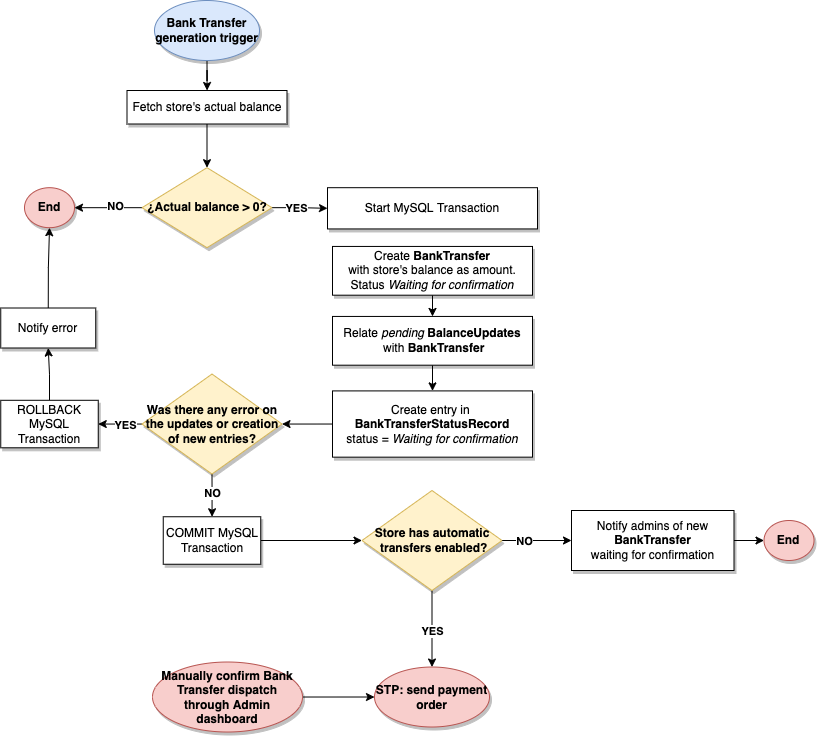
\includegraphics[scale = 0.4]{assets/flowcharts/BankTransferTrigger.png}
    \caption{Bank Transfers generating trigger}\label{fig:bank_Transfer_trigger}
\end{figure}

The process of actually sending the payment order through STP will be furtherly described in Chapter 4.\\

\subsubsection{Status updates records}

Every time that the internal status of a Balance Update or a Bank Transfer is updated a record will be generated to keep track of every update. As shown in previously shown diagrams, these records will be stored in the entities Bank Transfer Status Update Record and Balance Update Status Record respectively. Even though the status entities are equal in sturcture, they will be handled independently, for this reason the status updates records are handled independently as well.
These status records will simply keep track of the next status of any Balance Udpdate or Bank Transfer, as shown in Figure \ref{fig:status_record_uml} the creation date of the record will indicate the moment where the status was updated. For new instances of Balance Updates or Bank Transfers, a status record will be created with the initial status. 

\begin{figure} [H]
    \centering
    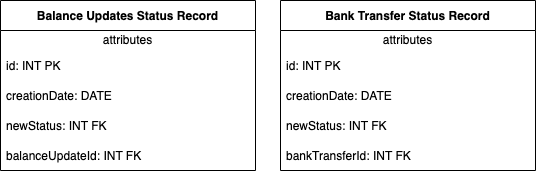
\includegraphics[scale = 0.6]{assets/uml/StatusRecordUML.png}
    \caption{Status Record UML for both Balance Updates and Bank Transfers}\label{fig:status_record_uml}
\end{figure}

Since a Bank Transfer is composed of multiple Balance Updates, then their status updates are directly related. Figure \ref{fig:bu_state_machine} describes how the status of any Balance Update could change depending on how the Bank Transfer's status changes. 

\begin{figure} [H]
    \centering
    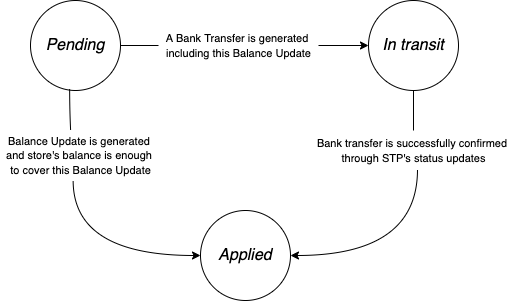
\includegraphics[scale = 0.6]{assets/diagrams/BUStateMachine.png}
    \caption{Balance Updates State Machine related to changes in their related Bank Transfers}\label{fig:bu_state_machine}
\end{figure}

Note how once a Balance Update is updated to the status \textit{Applied}, then it can not be updated furtherly; this is a final status. Any additional update regarding any confirmed Balance Update should be represented as a \textit{Cancelation}, Disbursement \textit{Cancelation} or \textit{Manual adjustment}, but the Balance Updated that was already applied will not produce any additional change in the store's balance.


\section{Ensure correct functionality and error handling through MySQL Transactions}

As noted in the diagrams exposed in previous sections, a particullar service from MySQL, called Transactions, is implemented for updating and inserting new entities to the databes. This database service, powered by Oracle, refers to a safe update functionality. These transactions enable running a group of statements, commonly used for inserting or updating data, with the possibility to discard all changes if required. This behaviour could be particularly usefeul when performing a large amount of updates or inserts within a large process. If any command fails for whatever reason, then all the previous updates should be rollbacked, resulting in a complete failed process instead of a partial failed process. Either every update is executed as expected or none of them are. The general structure of a MySQL Transaction is displayed in the following code snippet available from Oracle's official MySQL Reference Manual \cite{mysqldocs}

\begin{center}
    \begin{verbatim}
        START TRANSACTION;
        SELECT @A:=SUM(salary) FROM table1 WHERE type=1;
        UPDATE table2 SET summary=@A WHERE type=1;
        COMMIT;
    \end{verbatim}
\end{center}

Every transaction must start with the command \textit{START TRANSACTION}. Every following statement will run within the scope of the Transaction. Changes to the tables in the databse will not be made permanent immediately, since they must either commited or rollbacked. The \textit{COMMIT} statment will save the changes to disk while the \textit{ROLLBACK} command will ignore them. \cite{mysqldocs}\\

To enhance this funcionality and to make it compatible to the ORM Atrato is handling, a single connection must be assured will executing any transaction. TypeORM supports Transactions through the implementation of QueryRunners, specifically to create and control state of single database connection. A single QueryRunner instance must be created to handle a single Transaction.\cite{typeorm}\\ 

To instantiate a QueryRunner from TypeORM first the connection should be fetched. Once the QueryRunner is created and successfully created the single database connection, then the Transaction can be started. This process can be executed as follows:

\begin{verbatim}
    const connection = getConnection();
    const queryRunner = connection.createQueryRunner();
    await queryRunner.connect();
    await queryRunner.startTransaction();
\end{verbatim}

Once the transaction has been started within the scope of the QueryRunner, the correct Commit or Rollback should be handled appropiately. Once the transaction has been succesfully terminated, the Query Runner can be released.\cite{typeorm}

\begin{verbatim}
    // Only one of the following methods should be executed before releasing
    // the query runner
    await queryRunner.rollbackTransaction();
    await queryRunner.commitTransaction();
    // Release the single connection
    await queryRunner.release();
\end{verbatim}

The entire Balance System is composed by different events and triggers that could initiate specific processes where not only BalanceUpdates and BankTransfers, but also some Credit instances must be edited or added to the database. A correct functionality must be ensured and none of these processes should be partially completed. In other words, the creation and dispatch of a Bank Transfer must be donde successfully, with the corresponding state updates and records of these state changes. If an error occurs during any process, then the entities involved should not be edited, nor any additional entity should be created. The error could be later reviewed and the process could be repeated once again, replaced or even discarded. This expected behaviour also applies for handling the creation and update of the BalanceUpdates.\\

QueryRunners will be the base element managing all the updates and inserts within the complete Balance System. To apply correct design patterns and avoid repetition, a base controller class was developed to ensure that every method within the \textit{BankTransfersController} and the \textit{BalanceUpdatesController} could handle QueryRunners appropiately.

To ensure compatibility with Atrato's codebase and the Controllers' expected response, two methods where added in this base controller as described here: 

\subsubsection{Returning a successful Controller Response, handling the Commit and Release of the Query Runner's Transaction}

The method will take as a parameter the expected response to be returned and the Query Runner containing the single database connection. This method will simply assure that the existing Transaction will be commited and released before returning any successful response.

\begin{verbatim}
async returnSuccessWithCommit<T>(
       controllerSuccessfulResponse: T,
       queryRunner: QueryRunner
   ): Promise<{ success: true; res: T }> {
       await queryRunner.commitTransaction();
       await queryRunner.release();
       return { success: true, res: controllerSuccessfulResponse };
   }
\end{verbatim}

\subsubsection{Returning an unsuccessful Controller Response, handling the Rollback and Release of the Query Runner's Transaction}


Just like the successful response, the method will take as a parameter the Query Runner, but instead of having the expected response it will take as another argument the \textbf{\textit{controllerError}} created in any exception.

\begin{verbatim}
async returnErrorWithRollback(
       controllerError: ControllerError,
       queryRunner: QueryRunner
   ): Promise<{ success: false; error: ControllerError }> {
       await queryRunner.rollbackTransaction();
       await queryRunner.release();
       return { success: false, res: controllerError };
   }
\end{verbatim}

The combination of these methods compose the expected \textbf{\textit{ControllerResponse}} return interface for any Controller, as described at the begining of Chapter 3.

\section{Detailed visibility and traceability of full process}

The process being automated consists of very delicate matters, therefore, there should exist complete traceability of every action that was executed within the whole system. Every error presented during eny process should be able to be traced and identify easily in order ot take actions, as well as any process that was completed successfully. With this objective in mind, the Balance System was connected to an existing internal logging system, where every process interuption or completion is logged in the database with the respective data and payload necesary for identification.\\

Since all actinos regarding the database are hadndled through a QueryRunner, then this logging implementation should also considered these matters. Whenever process is completed and the changes will be commited, the log of this event should be included in the Commit. This applies equally for any action being rollbacked; the changes should e ignored by the trasnaction, but the log of the process should indeed be saved.

The logging system was integrated within the same Base Controller developed for handling Query Runners's transactions as follows:

For successful responses, the Log could be simply added as part of the existing transaction before commiting and releasing the connection as shown with pseudocode, refering to the implementation of the Successful and unsuccessful responses.

\begin{verbatim}
    async returnSuccessWithCommit<T>(
           controllerSuccessfulResponse: T,
           queryRunner: QueryRunner,
           processLog: Log
       ): Promise<{ success: true; res: T }> {
           // Save processLog to database
           await queryRunner.commitTransaction();
           await queryRunner.release();
           return { success: true, res: controllerSuccessfulResponse };
       }
\end{verbatim}

In the other hand, for unsuccessful responses the rollback should be done before adding anything extra to the trasnaction.  Once the trasnaction is rollbacked, the connection is still active, hence, normal statments can be executed which will be immediately applied.

\begin{verbatim}
    async returnErrorWithRollback(
           controllerError: ControllerError,
           queryRunner: QueryRunner.
           processLog: Log
       ): Promise<{ success: false; error: ControllerError }> {
           await queryRunner.rollbackTransaction();
           // Save processLog to database
           await queryRunner.release();
           return { success: false, res: controllerError };
       }
    \end{verbatim}

\section{Balance System Integration}

There are different events happening in Atrato's pipeline and business processes that could trigger some specific actions regarding the store's balance. The sytem could be affected either by updating the store's balance by adding new Balance Updates, or by generating bank Transfers objects from the existing Balance Updates. Furthermore, the status of these Bank Transfers could be updated, indicating some specific actions on the system. The existing events and triggers are shown in Figure \ref{fig:balance_system_triggers}.

\begin{figure}[H]
    \caption{Balance System Triggers}\label{fig:balance_system_triggers}
    \begin{tabularx}{1\textwidth} { 
    | >{\centering\arraybackslash}X 
    | >{\centering\arraybackslash}X 
    | >{\raggedright\arraybackslash}X | }
   \hline
   Event & Trigger & Description \\
   \hline
   \textit{Bank Transfer generation trigger} & Through Cron Job monitoring every store's disbursement type & Generates new Bank Transfer object with current's store balance [PENDIENTE]   \\
   \hline
   \textit{Contribution of new credit} & Notification of the delivery of a credit's product & Generates a Balance Update indicating the contribution to the stoere's balance  \\
   \hline
   \textit{Cancelation of credit} & Notification of the cancelation of a credit & Generates a Balance Update indicating the cancelation of the credit amount to the stoere's balance  \\
   \hline
   STP status update: \textit{Liquidated} & Through incoming activity in STP's webhook & Starts the confirmation process of a Bank Transfer   \\
   \hline
   STP status update: \textit{Cancelled} & Through incoming activity in STP's webhook & Starts the cancelation process of a Bank Transfer   \\
   \hline
   STP status update: \textit{Returned} & Through incoming activity in STP's webhook & Starts the rejection process of a Bank Transfer   \\
   \hline
\end{tabularx}
\end{figure}

    
Since most of these triggers happen as a result of automated processes or through actions from third parties, like merchants or STP's servive, to ensure the correct functionality of the balance system, Atrato must have a way of replicating these actions in case something external is not working as expected. Internally, any process executed as part of a web service or exposed endpoint to these third parties can also be executed by any administrator from Atrato with the required permissions.\\
    
The general integration of these events and triggers is described in Figure \ref{fig:balance_system_triggers}, displaying how the Balance Updates and the Bank Transfers in a Store's Balance System can be generated through distinct actions and how they relate between each other. Note how the only output of the system are the Bank Transfers generated as payment orders for the intrgration with STP's services Furthermore, STP will send updates on these payment ordrers' status and the system will then generate actions accordingly. Specifications on the integration with STP will be furtherly discussed in the following chapter.

\begin{figure} [H]
    \centering
    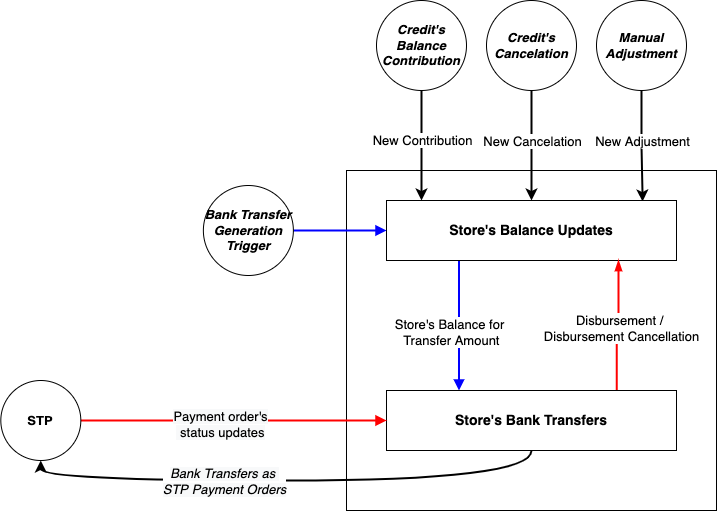
\includegraphics[scale = 0.5]{assets/diagrams/BalanceSystemDiagram.drawio.png}
    \caption{General integration of a Store's Balance System's triggers and internal processes}\label{fig:balance_systen_diaran}
\end{figure}

\section{Integration with current business processes}

Since the balance system is part of the general customer pipeline it must be directly integreated with current business processes. Once an application from a customer becomes an active credit, this credit could become part of the automated balance system of a store, depending if this store in particular has the automatic disbursements balance system enabled.\\

Furthermore, an existing credit could be affected through additinoal processes, like a change in the amount, a cancelation of the purchase or even a change of Store. The latter must be particularly addressed, since a credit could change from a store with its automatic system enabled to another one without it, or the other way around. The automation of any store's balance is completely integrated into every process to consider if the store has the system enabled or not before realizing any changes or updates to it. This behaviour is described in a general manner in Figure \ref{fig:automation_validation}, where this validation is included throughout every method of the Balance Updates and Bank Transfers Controllers.

\begin{figure} [H]
    \centering
    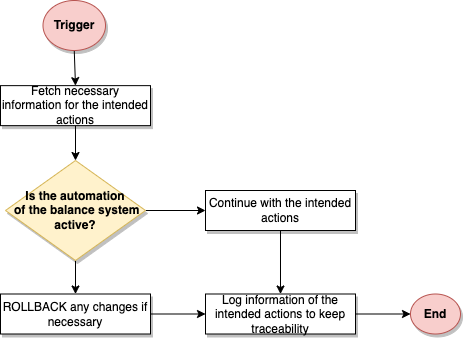
\includegraphics[scale = 0.5]{assets/flowcharts/AutomationValidation.png}
    \caption{General validation of Balance Updates and Bank Transfers Controllers' methods}\label{fig:automation_validation}
\end{figure}